\chapter{Wprowadzenie}

Rozwój technologiczny i informacyjny, zapoczątkowany w XX wieku, doprowadził do wytworzenia ogromnej ilości danych, które to nieustannie trwa do dziś, a ich ilość rośnie w~tempie wykładniczym. Sytuacja ta wymusiła powstanie nowych dziedzin nauki i inżynierii, zajmujących się przechowywaniem oraz przetwarzaniem tak licznych zbiorów danych (ang. \textit{big data}). W celu przeprowadzenia analizy i eksploracji danych oraz tworzenia, opartych o nie,  modeli statystycznych, sukcesywanie wykorzystywane są procedury statystyki matematycznej (opracowane już przed rewolucją informacyjną \cite{Robertson_1990}) na nieznaną wcześniej skalę. Wśród nich wyróżnia się:
\begin{enumerate}[label=(\alph*)] % (a), (b), (c), ...
\item \label{a} wykrywanie elementów nietypowych \cite{Aggarwal_2017, Barnett_1978} -- identyfikacja obserwacji (elementów zbioru danych), które znacznie różnią się od pozostałych,
\item klasteryzacja \cite{Xu_2008} -- grupowanie obserwacji w stosunkowo jednorodne podgrupy,
\item \label{c} klasyfikacja \cite{Duda_2000} -- przypisanie testowej obserwacji do jednej z wyróżnionych klas.
\end{enumerate}
Powyższe procedury są fundamentalnymi zagadnieniami w większości praktycznych zastosowań analizy i eksploracji danych \cite{Nisbet_2018}. Ponadto w wielu zastosowaniach procedury te stanowią dogodny szkielet koncepcyjny projektowanego rozwiązania \cite{Aggarwal_2015}. Wykrywanie elementów nietypowych pozwala na oczyszczenie danych z elementów odstających i~elementów obciążonych błędami grubymi, a w konsekwencji wprowadzających fałszywą informację \cite{Zieba_2013}. Klasteryzacja umożliwia podział danych na podzbiory podobnych elementów, dzięki czemu dalsza analiza przeprowadzana oddzielnie na jednorodnych podzbiorach staje się bardziej wydajna lub w ogóle możliwa. Z kolei klasyfikacja umożliwia przypisanie elementu -- będącego przedmiotem zainteresowania -- do jednej z wcześniej zdefiniowanych klas i dzięki temu wykorzystania tego elementu do wcześniej przygotowanej operacji, specyficznej względem owej klasy \cite{Kulczycki_2007}. Oczywiście każdy praktyczny problem wymaga zastosowania dodatkowych działań i indywidualnego podejścia \cite{Larose_2014}, jednakże procedury opisane w punktach \ref{a}--\ref{c} często stanowią istotne ramy wypracowanego rozwiązania. Ilustracja ich rezultatów, otrzymanych dla przykładowych danych syntetycznych w przestrzeni dwuwymiarowej, przedstawiona została na rysunku \ref{fig:intro}.

\begin{figure}
    \centering
    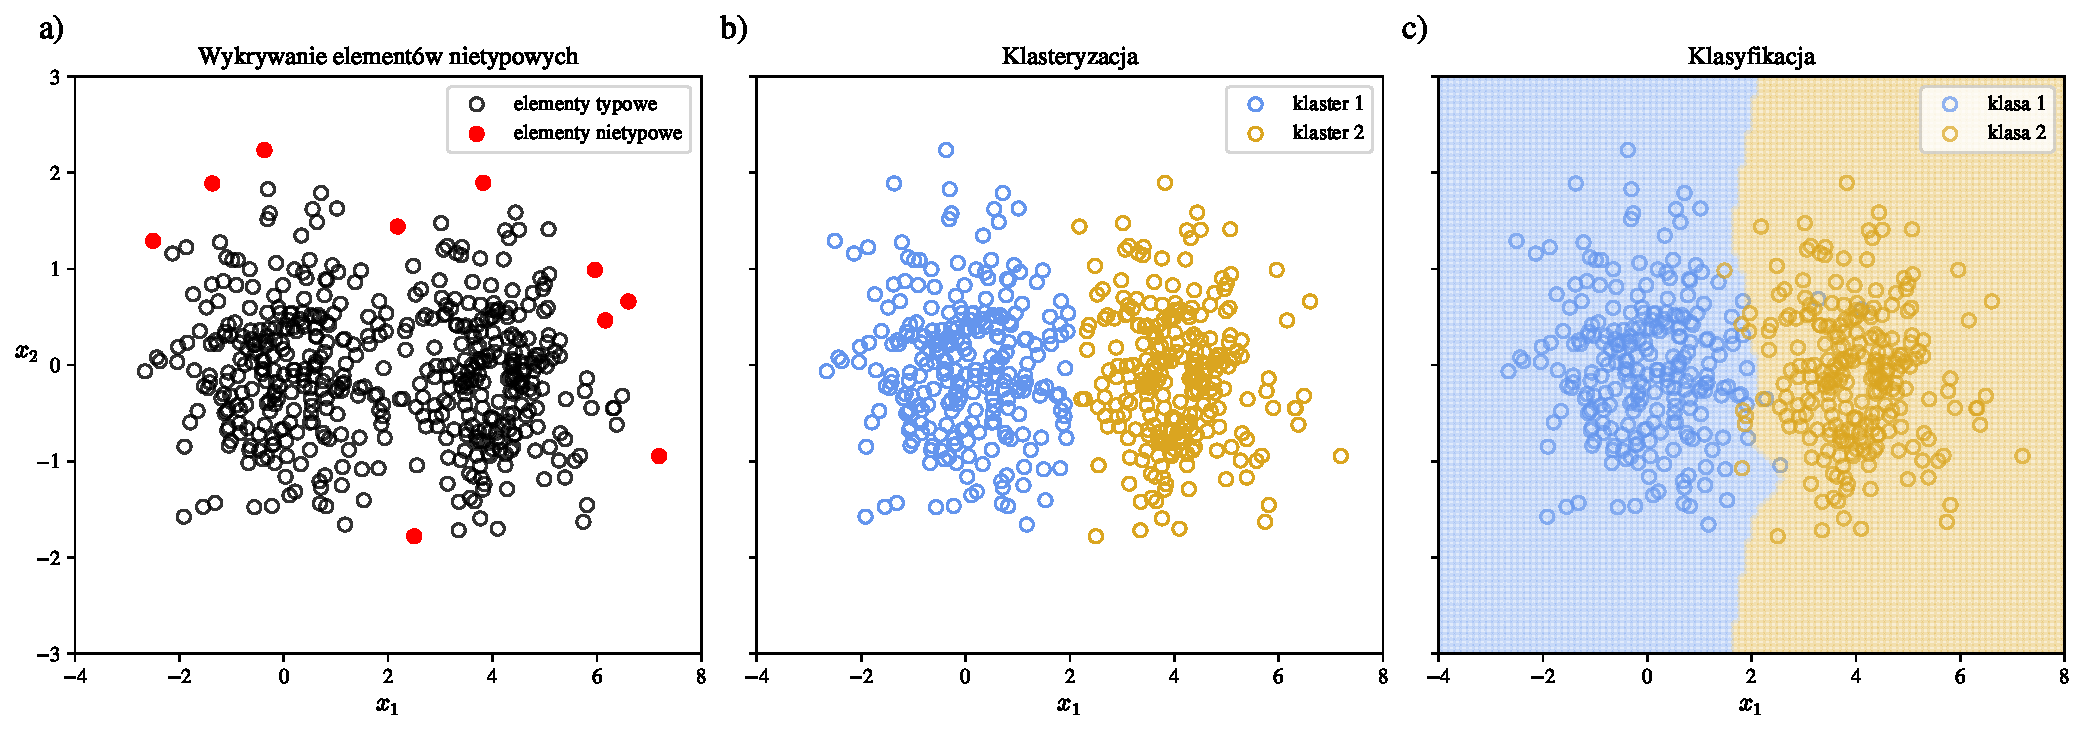
\includegraphics[scale=0.45]{intro}
    \vspace{-0.5cm} 
    \caption{Ilustracja przykładowych rezultatów procedur \ref{a}--\ref{c}.}
    \label{fig:intro}
\end{figure}

W wielu zadaniach praktycznych informacje zawarte w danych mogą zostać dodatkowo uściślone poprzez pomiar i wprowadzenie do modelu bieżących wartości czynników mających istotny wpływ na badane zjawisko. Takim czynnikiem może być na przykład aktualna temperatura w zagadnieniach inżynierskich lub dzień tygodnia w zagadnieniach marketingowych. Z formalnego punktu widzenia cel ten można osiągnąć przez zastosowanie probabilistycznego podejścia warunkowego \cite{Casella_2002}. Wówczas podstawowe atrybuty, nazywane objaśniajacymi, zależą od wartości warunkowych, których zmierzone i wprowadzone wartości mogą w znaczący sposób uściślić informacje dotyczące rozpatrywanego obiektu. \textbf{Takie podejście, zastosowane do procedur wykrywania elementów nietypowych, klasteryzacji i klasyfikacji, stanowi przedmiot niniejszej rozprawy}.

W celu określenia charakterystyk danych wykorzystana została nieparametryczna metoda estymatorów jądrowych \cite{Kulczycki_2005, Wand_1995}, która uwalnia badane procedury od założeń dotyczących postaci rozkładów prawdopodobieństwa charakteryzujących zarówno objaśniające, jak i warunkowe atrybuty. Koncepcja ta została wykorzystana w przypadku wszystkich trzech procedur \ref{a}--\ref{c}. Uzyskana w ten sposób jednorodność metodologii okazuje się bardzo cenna w praktycznych zastosowaniach. Uproszcza zrozumienie, interpretację, implementację i zgodność z indywidualnymi warunkami badawczymi, co jest warte szczególnego podkreślenia, zwłaszcza w kontekście współczesnych złożonych i interdyscyplinarnych zastosowań.

\textcolor{red}{Rozdział XXX niniejszej pracy przedstawia główne pojęcia teorii estymacji, natomiast wstępne zagadnienia matematyczne dotyczące statystycznych estymatorów jądrowych przedstawione zostały w rozdziale XXX. Procedury identyfikacji elementów nietypowych, klasteryzacji i klasyfikacji w podejściu warunkowym zostały opisane odpowiednio w rozdziałach XXX, XXX i XXX. Rozdział XXX prezentuje wyniki testów empirycznych, najpierw dla ilustracyjnych, sztucznie wygenerowanych danych (podrozdział XXX), a następnie dla zagadnień poczucia szczęścia (podrozdział XXX) i wreszcie dla badań z zakresu zanieczyszczeń środowiska (podrozdział XXX). Na zakończenie umieszczono uwagi końcowe oraz podsumowanie ninejszej pracy odpowiednio w rozdziałach XXX i XXX.}
